%!TEX TS-program = xelatex
\documentclass{EdipyLabs} % Custom class provided for EDIPY labs, by Christos Dalamagkas (cdalamagkas@gmail.com)
\SetLabNumber{4}
\SetLabTitle{Στατική Δρομολόγηση}
\SetAuthor{Χρήστος Δαλαμάγκας}
\SetLabDescription{Στατική δρομολόγηση, κανονική, προεπιλεγμένη, αθροιστική και εναλλακτική στατική διαδρομή, διαχειριστική απόσταση.}
\SetLabPrerequisites{Εργαστηριακά φυλλάδια 1β και 3 (Εισαγωγή στο RouterOS, Υποδικτύωση IPv4).}

\begin{document}
\Initialize

\section*{Εισαγωγή}
Αντικείμενο του παρόντος εργαστηριακού φυλλαδίου αποτελεί η εμβάθυνση στις τεχνικές στατικής δρομολόγησης για τη δημιουργία περισσότερο πολύπλοκων δικτύων. Η τοπολογία αποτελείται από δυο σενάρια με το πρώτο να αφορά την υλοποίηση εναλλακτικών στατικών διαδρομων (floating static routes) και το δεύτερο να εστιάζει στην τεχνική συνάθροισης διαδρομών. Η γενική άποψη της τοπολογίας φαίνεται στο σχήμα \ref{fig:topology}.

Για την υλοποίηση της τοπολογίας θα χρειαστείτε τις εξής συσκευές:
\begin{itemize}
	\item x2 δρομολογητές Cisco 2921
	\item x1 δρομολογητής MikroTik CCR-1009
	\item x2 μεταγωγείς Cisco Catalyst
	\item x3 υπολογιστές
\end{itemize}

\begin{figure}[ht]
	\centering
	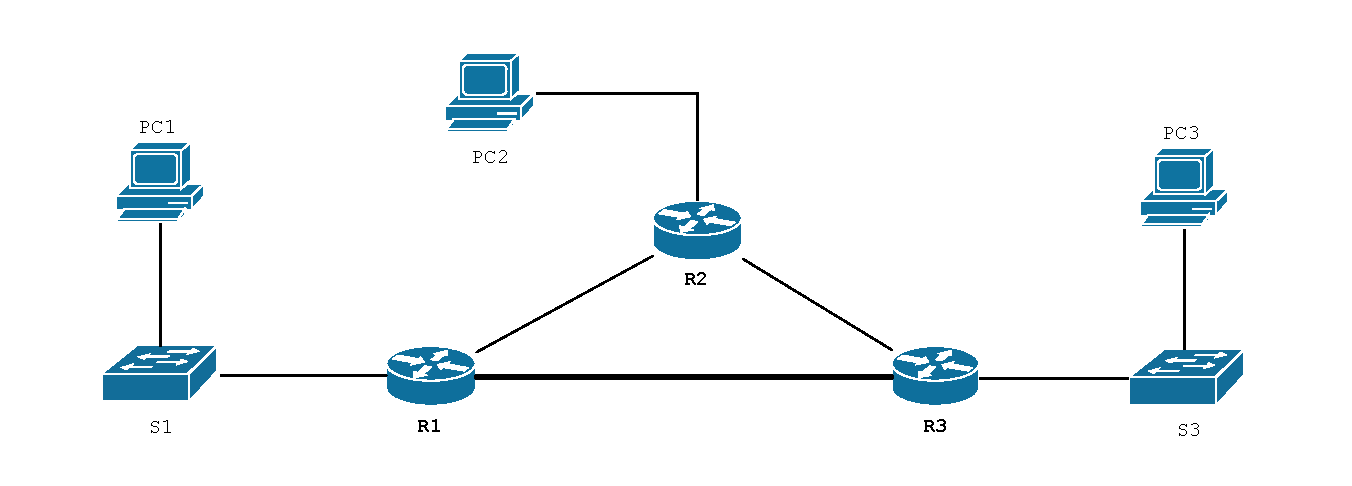
\includegraphics[width=\linewidth]{topology}
	\caption{H γενική άποψη της τοπολογίας προς υλοποίηση}\label{fig:topology}
\end{figure}

\section{Θεωρητικό υπόβαθρο}
Ο κυριότερος λόγος ύπαρξης των δρομολογητών είναι να διασυνδέουν απομακρυσμένα δίκτυα προωθώντας τα εισερχόμενα πακέτα προς τις κατάλληες διεπαφές, κάτι το οποίο επιτυγχάνουν χρησιμοποιώντας τους πίνακες δρομολόγησης. Για κάθε εισερχόμενο πλαίσιο, ο δρομολογητής καταστρέφει την επικεφαλίδα επιπέδου 2 (για παράδειγμα Ethernet ή PPP), εξάγει τη διεύθυνση IP προορισμού που περιέχεται στο ενθυλακωμένο πακέτο IP και την συγκρίνει με τις καταχωρήσεις του στον πίνακα δρομολόγησης. Αν βρεθεί κάποια αντιστοιχία, τότε το πακέτο προωθείται στην κατάλληλη διεπαφή.

Στο σχήμα \ref{fig:flow} απεικονίζεται το διάγραμμα ροής που ακολουθεί ένας δρομολογητής όταν λαμβάνει ένα πακέτο.\footnote{\itshape Πηγή σχήματος: Cisco Networking Academy.} Όπως φαίνεται και στο διάγραμμα, όταν ένας δρομολογητής λαμβάνει ένα πακέτο πρώτα ελέγχει αν αυτό προορίζεται σε \textbf{απευθείας συνδεδεμένο δίκτυο} (directly connected), δηλαδή δίκτυο στο οποίο ο δρομολογητής έχει δική του IP. Αν όχι, τότε ελέγχεται αν το πακέτο προορίζεται για \textbf{απομακρυσμένο δίκτυο}, δηλαδή δίκτυο στο οποίο ο δρομολογητής συνδέεται έμμεσα μέσω ενδιάμεσου δρομολογητή. Αν το πακέτο δεν προορίζεται ούτε προς απομακρυσμένο δίκτυο, τότε προωθείται στην πύλη δικτύου, αν υπάρχει, αλλιώς απορρίπτεται.

\begin{figure}[ht]
	\centering
	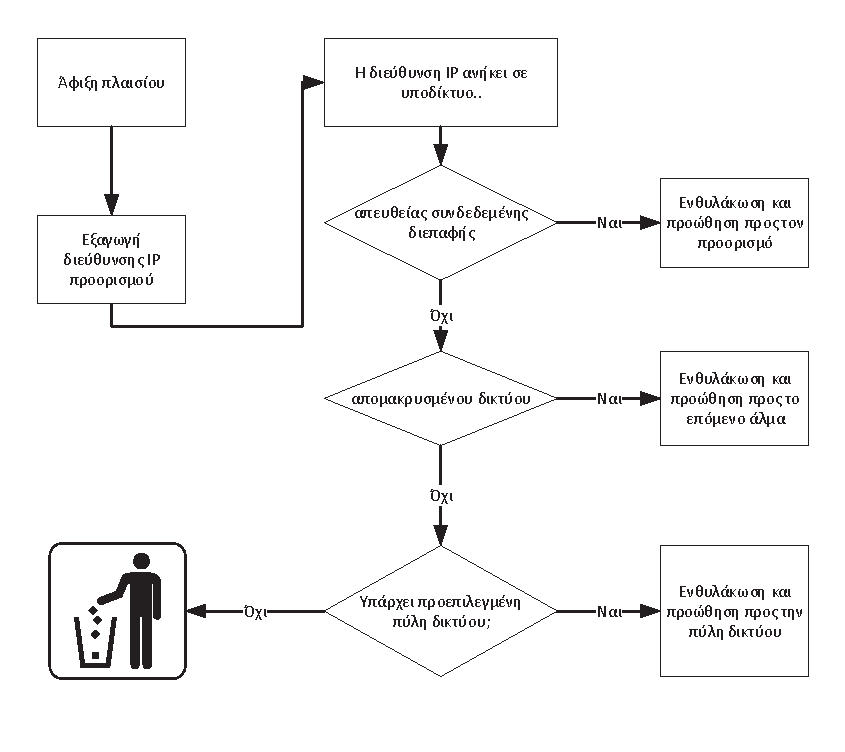
\includegraphics[width=\linewidth]{flow}
	\caption{To διάγραμμα ροής για την απόφαση προώθησης εισερχόμενου πακέτου.}\label{fig:flow}
\end{figure}

Ένας δρομολογητής μαθαίνει απομακρυσμένα δίκτυα είτε με στατικό τρόπο, δηλαδή μέσω χειροκίνητων καταχωρήσεων του διαχειριστή δικτύου στον πίνακα δρομολόγησης, είτε δυναμικά μέσω διαφημίσεων που λαμβάνει ο δρομολογητής από πρωτόκολλα δυναμικής δρομολόγησης. 

Δύναται ένας δρομολογητής να γνωρίζει περισσότερες από μια διαδρομές για ένα απομακρυσμένο δίκτυο. Σε αυτή την περίπτωση, ο δρομολογητής επιλέγει τη διαδρομή με τη μικρότερη \textbf{διαχειριστική απόσταση} (administrative distance) για το Cisco IOS ή απλά \textbf{απόσταση} για το RouterOS. Η διαχειριστική απόσταση ορίζεται ως η αξιοπιστία μιας διαδρομής (trustworthiness), η οποία εξαρτάται από το πρωτόκολλο δρομολόγησης. Στα έγγραφα του εργαστηρίου παρατίθενται οι προεπιλεγμένες αποστάσεις για κάθε πρωτόκολλο δρομολόγησης.

Στον πίνακα δρομολόγησης απεικονίζεται μόνο η διαδρομή που επικρατεί για τον εκάστοτε προορισμό. Δηλαδή, ένας δρομολογητής μπορεί να διαθέτει πολλαπλές διαδρομές για έναν προορισμό με διαφορετικές αποστάσεις, ωστόσο μόνο η διαδρομή με τη χαμηλότερη διαχειριστική απόσταση και ενεργοποιημένη την αντίστοιχη διεπαφή εξόδου εμφανίζεται στον πίνακα δρομολόγησης και λαμβάνεται υπόψιν από τον δρομολογητή για τη λήψη της απόφασης προώθησης ενός πακέτου. 

Για μικρά δίκτυα, η τοπολογία των οποίων παραμένει σταθερή, η στατική δρομολόγηση αποτελεί μια απλή και εφικτή λύση για την επικοινωνία απομακρυσμένων δικτύων. Η στατική δρομολόγηση, η οποία υλοποιείται με εντολές του διαχειριστή, δεν καταναλώνει επεξεργαστικούς πόρους από τους δρομολογητές, ούτε εύρος ζώνης από τις ζεύξεις, συνεπώς εισάγει τις μικρότερες δυνατές καθυστερήσεις κατά τη δρομολόγηση. Τα είδη στατικών διαδρομών που μπορούν να προστεθούν σε έναν δρομολογητή συνοψίζονται στα εξής:
\begin{itemize}
	\item \textbf{Κανονική} στατική διαδρομή (standard static route): Είναι η διαδρομή που έχει ως διεύθυνση προορισμού ένα συγκεκριμένο απομακρυσμένο δίκτυο. 
	\item \textbf{Προεπιλεγμένη} στατική διαδρομή (default static route): Είναι η διαδρομή που έχει ως διεύθυνση προορισμού το δίκτυο \ip{0.0.0.0/0}, δηλαδή «όλα τα δίκτυα». Η συγκεκριμένη στατική διαδρομή ελέγχεται τελευταία, μετά από οποιαδήποτε άλλη διαδρομή. 
	\item \textbf{Αθροιστική} στατική διαδρομή (summary static route): Είναι η διαδρομή που περιέχει ένα υπερδίκτυο (supernet), δηλαδή ένα δίκτυο με μεγαλύτερη μάσκα, ώστε να περιλαμβάνει πολλά υποδίκτυα της τοπολογίας. Χρησιμεύει για τη μείωση της έκτασης ενός πίνακα δρομολόγησης, αλλά και του φόρτου του διαχειριστή που δίνει τις εντολές στατικής δρομολόγησης.
	\item \textbf{Εναλλακτική} στατική διαδρομή (floating static route): Είναι μια στατική διαδρομή με υψηλότερη απόσταση από την προεπιλεγμένη, με σκοπό να επιλεγεί από τον δρομολογητή, αν η πρωτεύουσα διαδρομή αποτύχει. Στα αγγλικά οι εναλλακτικές διαδρομές αποκαλούνται «επιπλέουσες», διότι «αναδύονται» όταν οι διαδρομές με χαμηλότερη απόσταση προς τον ίδιο προορισμό δεν είναι διαθέσιμες.
\end{itemize}
\newpage

\section{Προετοιμασία δικτύου}

\begin{figure}[H]
	\centering
	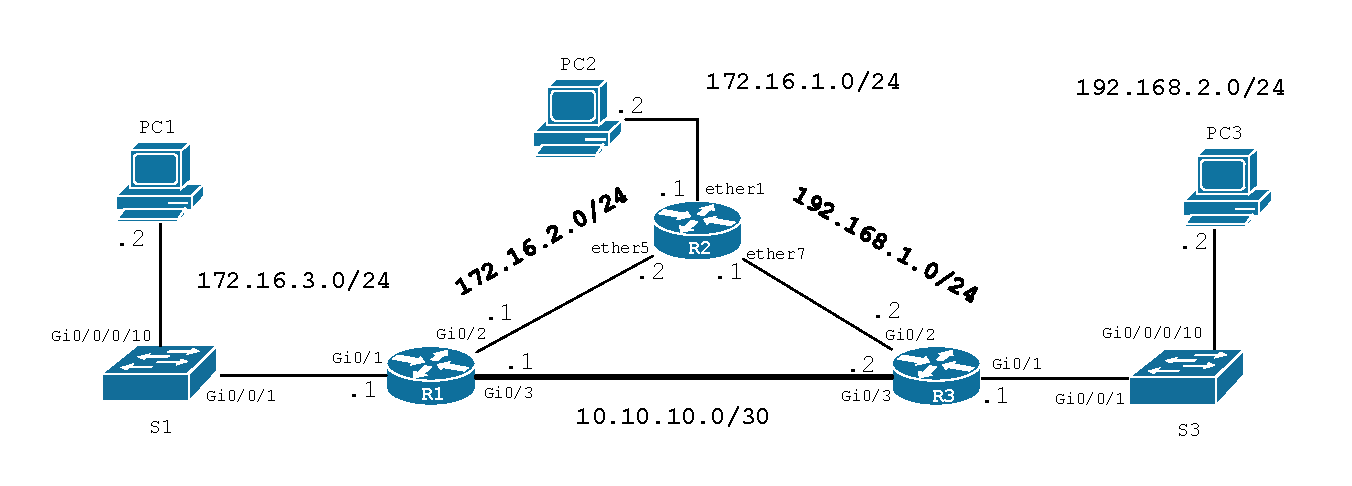
\includegraphics[width=\linewidth]{topology1}
	\caption{Το σχέδιο της αναλυτικής τοπολογίας προς υλοποίηση.}\label{fig:topology1}
\end{figure}

\begin{IpAddressTable}{Σχήμα διευθυνσιοδότησης της τοπολογίας.}{addr}
						& Gi0/0		& 172.16.3.1	& 255.255.255.0 	& \\
						& Gi0/1		& 172.16.2.1	& 255.255.255.0 	& \\
\multirow{-3}{*}{R1}	& Gi0/2		& 10.10.10.1	& 255.255.255.252 	& \multirow{-3}{*}{-} \\
\rowcolor{lightgray}	& ether1	& 172.16.1.1	& 255.255.255.0 	& \\
\rowcolor{lightgray}	& ether5	& 172.16.2.2	& 255.255.255.0 	& \\
\rowcolor{lightgray}
\multirow{-3}{*}{R2}	& ether7	& 192.168.1.1	& 255.255.255.0 	& \multirow{-3}{*}{-}\\
						& Gi0/0		& 192.168.2.1	& 255.255.255.0 	& \\
						& Gi0/1		& 192.168.1.2	& 255.255.255.0 	& \\
\multirow{-3}{*}{R3}	& Gi0/2		& 10.10.10.2	& 255.255.255.252 	& \multirow{-3}{*}{-}\\
\rowcolor{lightgray}PC1 & \NIC		& 172.16.3.2	& 255.255.255.0 	& 172.16.3.1\\
		PC2				& \NIC		& 172.16.1.2	& 255.255.255.0		& 172.16.1.1\\
\rowcolor{lightgray}PC3 & \NIC		& 192.168.2.2	& 255.255.255.0 	& 192.168.2.1

\end{IpAddressTable}

Ακολουθήστε τα εξής βήματα για την προετοιμασία του δικτύου της εργαστηριακής άσκησης:
\begin{itemize}
	\item Υλοποιήστε τη συνδεσμολογία που απεικονίζεται στο σχήμα της τοπολογίας. Για το υπόλοιπο της άσκησης, θεωρήστε πως ο δρομολογητής \textbf{MikroTik} είναι ο \textbf{R2}.
	\item Βεβαιωθείτε ότι όλες οι δικτυακές συσκευές λειτουργούν στις εργοστασιακές ρυθμίσεις. Συμβουλευτείτε τα εισαγωγικά φυλλάδια για το Cisco IOS και το RouterOS για τις κατάλληλες εντολές.
	\item Αναθέστε διευθύνσεις IP στους υπολογιστές και τους δρομολογητές, σύμφωνα με το σχήμα διευθυνσιοδότησης. Για τον δρομολογητή MikroTik εκτελέστε τις εντολές που ακολουθούν για την επιθυμητή ρύθμιση IP:
\begin{CommandBox}
[admin@MikroTik] > `\textbf{system identity set name=R2}`
[admin@R2] > `\textbf{ip address}`
[admin@R2] ip address> `\textbf{add address=172.16.2.2/24 interface=ether5}`
[admin@R2] ip address> `\textbf{add address=172.16.1.1/24 interface=ether1}`
[admin@R2] ip address> `\textbf{add address=192.168.1.1/24 interface=ether7}`
[admin@R2] ip address> 
\end{CommandBox}
	\item Αν κρίνετε ότι χρειάζεται, επιβεβαιώστε με την εντολή \ip{ping} τη σωστή παραμετροποίηση των διεπαφών για τις συνδέσεις σημείου προς σημείο.
\end{itemize} 

\section{Κανονικές στατικές διαδρομές}

Ξεκινώντας από τον R1, τα απομακρυσμένα δίκτυα προορισμού που δεν γνωρίζει και χρειάζεται να γνωρίζει ο δρομολογητής είναι τα 172.16.1.0/24 και 192.168.2.0/24. Ο δρομολογητής δεν χρειάζεται να γνωρίζει κάτι περισσότερο για τα δίκτυα αυτά, πέρα από την ταυτότητα του καθενός μαζί με τη μάσκα του, καθώς και τη διεπαφή που πρέπει να επιλέξει, ή τη διεύθυνση IP του «απέναντι» δρομολογητή, για να προωθήσει ένα πακέτο, ώστε αυτό να φτάσει στο προορισμό του.

Παρατηρώντας την τοπολογία, φαίνεται ότι ο R1 μπορεί να προσεγγίσει το απομακρυσμένο δίκτυο \ip{172.16.1.0/24} μέσω της ζεύξης του απευθείας συνδεδεμένου δικτύου 172.16.2.0/24, στο οποίο δίκτυο το επόμενο άλμα (R2) έχει τη διεύθυνση 172.16.2.2. Ακόμη, ο R1 μπορεί να προσεγγίσει το απομακρυσμένο δίκτυο \ip{192.168.2.0/24} μέσω της ζεύξης του απευθείας συνδεδεμένου δικτύου 10.10.10.0/24, στο οποίο δίκτυο το επόμενο άλμα (R3) διαθέτει τη διεύθυνση 10.10.10.2. Δώστε, λοιπόν, τις ακόλουθες εντολές \texttt{ip route} στον R1 για να συμπληρώσετε κατάλληλα τον πίνακα δρομολόγησής του:

\begin{CommandBox}
R1(config)#`\textbf{ip route 172.16.1.0 255.255.255.0 172.16.2.2}`
R1(config)#`\textbf{ip route 192.168.2.0 255.255.255.0 10.10.10.2}`
R1(config)#
\end{CommandBox}

Η εντολή \texttt{ip route} για το Cisco IOS συντάσσεται ως εξής. Ως επόμενο άλμα μπορεί να επιλεγεί είτε η διεπαφή εξόδου είτε ο επόμενος δρομολογητής που πρέπει να παραλάβει το πακέτο που προωθείται. Για μέσα πολλαπλής πρόσβασης, όπως το ethernet, προτείνεται η χρήση IP επόμενου άλματος, ενώ για σειριακές διεπαφές προτείνεται ο ορισμός διεπαφής εξόδου.

\begin{CommandBox}
Router(config)#`\textbf{ip route} \textit{dest-network} \textit{mask} \{\textit{next\_hop} | \textit{interface}\}`
\end{CommandBox}

Στη συνέχεια, δώστε τις ακόλουθες εντολές στατικής δρομολόγησης, ώστε ο δρομολογητής R2 να προωθεί πακέτα που προορίζονται για τα απομακρυσμένα δίκτυα που δε γνωρίζει (192.168.2.0/24 και 172.16.3.0/24) προς τον κατάλληλο δρομολογητή επόμενου άλματος.

\begin{CommandBox}
[admin@R2] ip address> `\textbf{.. route}`
[admin@R2] ip route> `\textbf{add dst-address=192.168.2.0/24 gateway=192.168.1.2}`
[admin@R2] ip route> `\textbf{add dst-address=172.16.3.0/24 gateway=172.16.2.1}`
[admin@R2] ip route> 
\end{CommandBox}

Δώστε τις κατάλληλες εντολές στον R3, ώστε να προσθέσετε στον πίνακα δρομολόγησής του τα άγνωστα για εκείνον απομακρυσμένα δίκτυα. Θεωρήστε ότι ο R3 προσεγγίζει το δίκτυο 172.16.3.0/24 μέσω της σύνδεσης σημείου προς σημείο με τον R1 και το δίκτυο 172.16.1.0/24 απευθείας μέσω του R2.

\subsection*{Δοκιμές συνδεσιμότητας}
Έχοντας υλοποιήσει πλήρως το δικτύωμα, πραγματοποιήστε τις απαραίτητες δοκιμές συνδεσιμότητας. Χρησιμοποιήστε το πρόγραμμα \ip{tracert} από τον κάθε υπολογιστή για να φτάσετε στους υπολογιστές των έτερων απομακρυσμένων δικτύων. Επιβεβαιώστε ότι το κάθε πακέτο ακολουθεί την προβλεπόμενη διαδρομή.

\section{Σενάριο: Εναλλακτικές διαδρομές}

Σύμφωνα με τις εντολές στατικής δρομολόγησης που έχουν εισαχθεί στους δρομολογητές R1 και R3, γίνεται εμφανές ότι σε περίπτωση που η απευθείας σύνδεση των R1 και R3 διακοπεί, δεν είναι δυνατή η επικοινωνία των δυο δρομολογητών, παρόλο που υπάρχει ο ενδιάμεσος δρομολογητής R2.

Για να αντιμετωπίσετε αυτό το πρόβλημα, μπορείτε να εισάγετε εναλλακτικές διαδρομές (floating static routes) στους δυο δρομολογητές, ώστε οι R1 και R3 να προτιμούν τον R2 για τα δίκτυα 172.16.3.0/24 και 192.168.2.0/24 στην περίπτωση που η πρωτεύουσα διαδρομή δεν είναι διαθέσιμη. Για να λειτουργήσουν αυτές οι διαδρομές ως εναλλακτικές θα πρέπει να έχουν διαχειριστική απόσταση μεγαλύτερη από αυτή των κανονικών στατικών διαδρομών

Για το Cisco IOS μπορείτε να προσδιορίσετε τη διαχειριστική απόσταση χρησιμοποιώντας της εντολή \texttt{ip route} με την εξής σύνταξη:

\begin{CommandBox}
Router(config)#`\textbf{ip route} \textit{dest-network} \textit{mask} \{\textit{next\_hop} | \textit{interface}\} distance`
\end{CommandBox}

Για να οριστεί μια διαδρομή εναλλακτική μιας κύριας διαδρομής θα πρέπει να έχει διαχειριστική απόσταση μεγαλύτερη από αυτή της κύριας. Δεδομένου ότι η προεπιλεγμένη απόσταση για τις στατικές διαδρομές είναι 1, η απόσταση της εναλλακτικής της πρέπει να είναι μεγαλύτερη του ενός. 

Από τον δρομολογητή R1 δώστε την εξής εντολή για να ορίσετε ως εναλλακτική διαδρομή του 192.168.2.0/24 αυτή μέσω του R2, με διαχειριστική απόσταση 5:

\begin{CommandBox}
R1(config)#`\textbf{ip route 192.168.2.0 255.255.255.0 172.16.2.2 5}`
\end{CommandBox}

Από τον δρομολογητή R3 δώστε την εξής εντολή για να ορίσετε ως εναλλακτική διαδρομή του 172.16.3.0/24 αυτή μέσω του R2, με διαχειριστική απόσταση 5:

\begin{CommandBox}
R3(config)#`\textbf{ip route 172.16.3.0 255.255.255.0 192.168.1.1 5}`
\end{CommandBox}

Προκαλέστε πτώση της σύνδεσης μεταξύ των R1 και R3, απενεργοποιώντας τη διεπαφή G0/2 ενός εκ των δυο δρομολογητών με την εντολή \ip{shutdown}. Εναλλακτικά, μπορείτε να αφαιρέσετε το καλώδιο που συνδέει τους δρομολογητές. Προβάλλοντας τους πίνακες δρομολόγησης, θα πρέπει να δείτε τις εναλλακτικές διαδρομές που ορίσατε για τους R1 και R3. Εκτελέστε την \ip{tracert} για να επιβεβαιώσετε πως υπάρχει ακόμα επικοινωνία μεταξύ των δικτύων μέσω των εναλλακτικών διαδρομών.

\begin{CommandBox}
R1>`\textbf{show ip route | begin Gateway}`
Gateway of last resort is not set
	
     172.16.0.0/16 is variably subnetted, 5 subnets, 2 masks
S       172.16.1.0/24 [1/0] via 172.16.2.2
C       172.16.2.0/24 is directly connected, GigabitEthernet0/1
L       172.16.2.1/32 is directly connected, GigabitEthernet0/1
C       172.16.3.0/24 is directly connected, GigabitEthernet0/0
L       172.16.3.1/32 is directly connected, GigabitEthernet0/0
`\hl{S}`       `\hl{192.168.2.0/24 [5/0] via 172.16.2.2}
\end{CommandBox}

Τέλος, επαναφέρετε τη σύνδεση μεταξύ των δυο δρομολογητών ενεργοποιώντας τη διεπαφή που απενεργοποιήσατε ή επανασυνδέοντας το καλώδιο. Οι πίνακες δρομολόγησης θα πρέπει να δείχνουν τις αρχικές στατικές διαδρομές με διαχειριστική απόσταση 1.

\section{Σενάριο: Συνάθροιση διαδρομών}

Βασικό μειονέκτημα της στατικής δρομολόγησης είναι ο φόρτος, τον οποίον επωμίζονται οι διαχειριστές για την παραμετροποίηση ενός δικτύου, ο οποίος μάλιστα πολλαπλασιάζεται για κάθε LAN που προστίθεται στην τοπολογία. Ωστόσο, η κατάλληλη επιλογή διευθύνσεων IP και ανάθεσή τους με τοπολογικά κριτήρια μπορεί να μειώσει αισθητά τον απαιτούμενο φόρτο.

Παρατηρώντας τη διευθυνσιοδότηση της τοπολογίας στο σχήμα \ref{fig:topology1}, είναι εμφανές ότι τα δίκτυα 172.16.1.0/24, 172.16.2.0/24 και 172.16.3.0/24 βρίσκονται σε γειτονικούς δρομολογητές. Αναπαριστώντας τα δίκτυα αυτά στο δυαδικό, διαπιστώνει κάποιος πως διαφέρουν μόνο κατά δυο bit.

\begin{tabular}{cc}
	\texttt{172.16.1.0} & \texttt{\hl{10101100.00010000.000000}01.00000000}\\
	\texttt{172.16.2.0} & \texttt{\hl{10101100.00010000.000000}10.00000000}\\
	\texttt{172.16.3.0} & \texttt{\hl{10101100.00010000.000000}11.00000000}
\end{tabular}

Συνεπώς, το ελάχιστου μεγέθους δίκτυο, στο οποίο μπορούν να συμπεριληφθούν τα συγκεκριμένα υποδίκτυα, είναι το 172.16.0.0/22.

Ελαχιστοποιώντας, λοιπόν, τον πίνακα δρομολόγησης του R3 μπορείτε να αφαιρέσετε τις στατικές διαδρομές για τα δυο υποδίκτυα και να τις αντικαταστήσετε από μια αθροιστική στατική διαδρομή για το υπερδίκτυο, με επόμενο άλμα τον R1 ή τον R2. Δώστε τις εντολές που ακολουθούν στον R3:

\begin{CommandBox}
R3(config)#`\textbf{no ip route 172.16.1.0 255.255.255.0 172.16.2.2}`
R3(config)#`\textbf{no ip route 192.168.2.0 255.255.255.0 10.10.10.2}`
R3(config)#`\textbf{ip route 172.16.0.0 255.255.252.0 10.10.10.1}`
\end{CommandBox}

Βασικές προυποθέσεις για να εφαρμοστεί η τεχνική συνάθροισης διαδρομών είναι το μπλοκ των διευθύνσεων των απομακρυσμένων δικτύων να είναι συνεχόμενο και τα υποδίκτυα να βρίσκονται σε συσκευές με άμεση τοπολογική σύνδεση. 

\end{document}
